\chapter{Fortbewegung, Lokalisierungsalgorithmen}
\section{Relative Lokalisierung}
\subsection{Dead Reckoning}
\begin{itemize}
	\item \textbf{Koppelnavigation oder Dead Reckoning} ursprünglich in der Nautik verwendet
	\item Mathematisches Verfahren - \textbf{Vorwärtskinematik} - zur Positionsbestimmung
	\item Ausgehend von einer Startposition ist es dem Navigator möglich, seine \textbf{aktuelle Position zu berechnen} aufgrund der \textbf{zurückliegenden bekannten Kurs- und Geschwindigkeitswerte}
\end{itemize}
\begin{figure}[H]
	\begin{center}
		\includegraphics[scale=0.7]{Resources/PDF/deadreckoning.pdf}
		\caption{}
		\label{fig:PDF/deadreckoning.pdf}
	\end{center}
\end{figure}
\begin{itemize}
	\item A sei ein gegebener Ausgangspunkt
	\item Radius wird angegeben der zur Abweichung proportional ist, bsp. hier 0,5m.
	\item Der Radius spiegelt die mit der Zeit kumulierte Ungenauigkeit wieder
	\item Eine mögliche Roboterposition ist dann innerhalb des Sektors gegeben der durch die Linien eingegrenzt wird
\end{itemize}
\paragraph{Vorteile}
\begin{itemize}
	\item einfache Implementierung
	\item leichte Interpretation der Daten
	\item unkomplizierte Bedienung
	\item passable Kurzstreckengenauigkeit
\end{itemize}
\paragraph{Nachteile}
\begin{itemize}
	\item Startposition muss bekannt sein
	\item Genauigkeit nimmt mit zunehmender Länge der befahrenen Strecke drastisch ab
\end{itemize}
\subsection{Odometrie}
Odometrie ist die Wissenschaft der Positionsbestimmung eines Fahrzeugs durch die Beobachtung seiner Räder.
\paragraph{Grundlegendes verfahren}
\begin{itemize}
	\item Sensoren an Rädern messen Drehbewegung
	\item \textbf{Relative Positionsbestimmung:} Die \textbf{Bestimmung der Position} erfolgt ausgehend von einer bekannten Position durch Berechnung des zurückgelegten Weges und anhand von Daten über den Roboter selbst.
	\item Es wird Inkrementalgebern die Anzahl $n$ der Radumdrehungen zwischen zwei Messpunkten gezählt. Aus dem bekannten Radumfang wird die wegdifferenz berechnet mit:
	\subitem $\Delta = \Pi \times d \times n $
	\item \textbf{Ausrichtung} kann durch differentiale Odometrie erfolgen: es werden z.B. die unterschiedlichen Entfernungen gemessen, die die linken und rechten Räder zurückgelegt haben.
\end{itemize}
\paragraph{Vorteile}
\begin{itemize}
	\item kostengünstig
	\item hohe Abtastraten
	\item passable Kurzzeitgenauigkeit
\end{itemize}
\paragraph{Fehlerquellen}
\begin{itemize}
	\item Fehlerhafte Messung des Raddurchmessers
	\item Raddurchmesser nicht gleich, Unrundheit des Radess
\end{itemize}
\paragraph{Fehlerberücksichtigung}
\begin{itemize}
	\item Die \textbf{Fehler} fließen in die Positionsdifferenz ein, werden zur letzten bekannten Position hinzuaddiert und \textbf{summieren sich mit jedem Messschritt}
	\item Fehlerellipse wächst mit zurückgelegtem Weg
	\item Odometrie als alleiniges verfahren nur für kurze Strecken geeignet
	\item Fehler lassen sich bei geringen Geschwindigkeiten und geringer Beschleunigung reduziern
\end{itemize}
\subsection{2D-Scanmatching}
\begin{itemize}
	\item Ausgangslage sind zwei Scans, ein Scan M (\textbf{Modell}) und ein zweiter Scan D (\textbf{Daten})
	\item Es wird eine Transformation des einen Scans berechnet und zwar so, dass beide optimal überlagert werden
	\item Die Transformationen bestehen nur aus einer Rotation und einer Translation
	\item Die Überlagerung ist optimal, wenn Punkte, die in der realen Szene nahe beieinander liegen, auch in den registrierten Messdaten nahe beieinander liegen.
	\item \textbf{Ziel}: Fehlerfunktion minimieren $\Rightarrow$ Abstände der Punkte des einen Scans zu ihren korrespondierenden Punkten des zweiten Scans
	\item Die Transformation des zweiten Scans entspricht dann der Bewegung des Roboters zwischen der Aufnahme der Daten; durch sukzessiven Vergleich kann damit die Bewegung des Roboters nachverfolgt werden
\end{itemize}
%TODO Rework this after understanding it
\paragraph{Iteratives Vorgehen}
\begin{figure}[]
	\begin{center}
		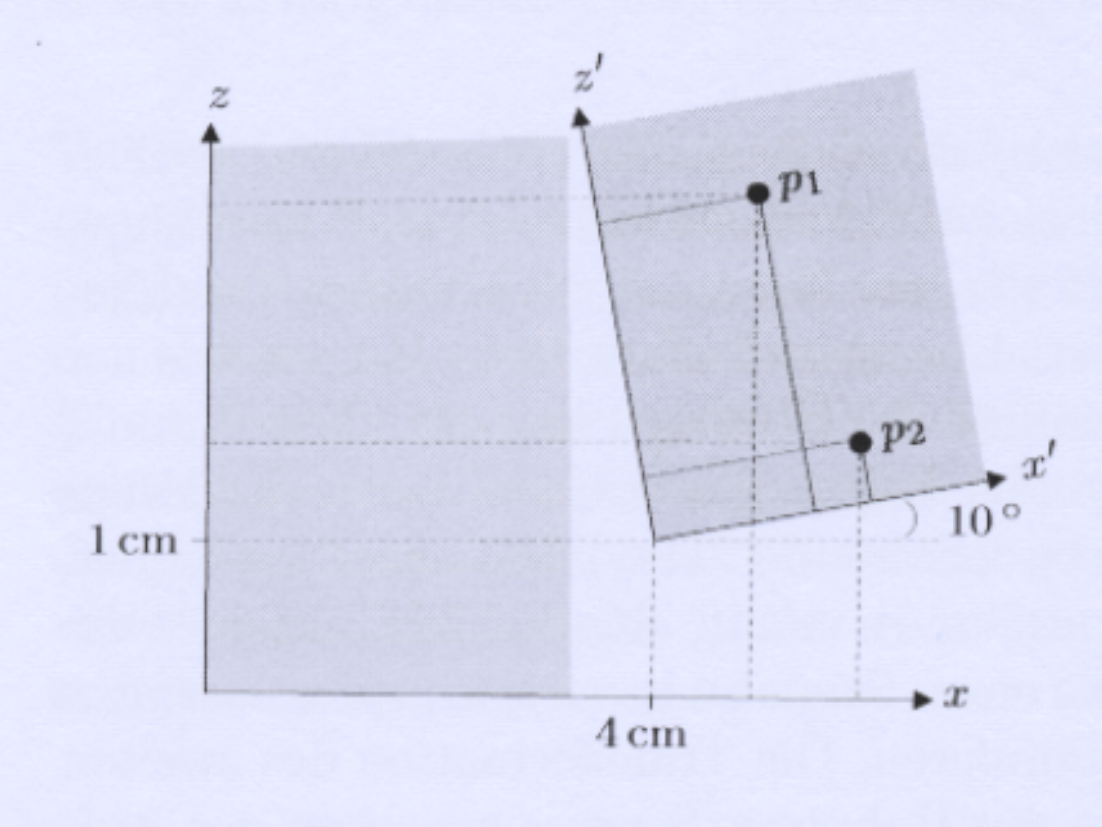
\includegraphics[scale=0.3]{Resources/PNG/2DScan.PNG}
		\caption{}
		\label{fig:PNG/2DScan.PNG}
	\end{center}
\end{figure}	
\begin{itemize}
	\item \textbf{Annahme:} die korrespondierenden Punkte sind bekannt $\Rightarrow$ eine \textbf{Transformation} kann berechnet werden, die diese Mengen aufeinander abbildet
	\item \textbf{Beispiel} zwei Scans mit einer Poseänderung des zweiten um $(4cm, 1cm, 10 \deg)^T$ beide Scans sehen dieselben Raumpunkte p1 und p2
	\item Obige Annahme i.d.r. nicht erfüllt $\Rightarrow$ \textbf{nicht eindeutig zu bestimmen, welche Punkte zwischen den beiden Scans korresponideren}
	\item \textbf{Lösung}: \textbf{iteratives Vorgehen}, bei dem zunächst eine \textbf{Schätzung} der Punktepaarung stattfinden und die Pose des zweiten Scans unter dieser Paarung optimiert wird.
	\item Iterativ werden mit dem transformierten Scan neue Punktepaare berechnet, bis ein Abbruchkriterium erfüllt ist, d.h. bis sich die Transformation zwischen zwei Schritten nich mehr signifikant ändert
\end{itemize}
\paragraph{Transformationsberechnung}
\begin{itemize}
	\item \textbf{Gesucht}: Mögliche Menge von Translationen und Rotationen, unter denen ein korrektes Matching möglich ist.
	\item $(t_x, t_z, \theta)^T$, die eine Translation um $t_x$ in x-Richtung und $t_z$ entlang der Z-Achse durchführt, sowie eine Rotation um den Winkel $\theta$
	\item Der Scan M besteht aus einer Menge von Punkten ($m_i$)i=1,2...N
	\item Der Scan D besteht aus einer Menge von Punkten ($D_i$)i=1,2...N
\end{itemize}
\paragraph{Minimum der Funktion}
$E(\theta, t)=\sum_{i=1}^{N}\left\|p_{i}-\left(\boldsymbol{R}_{\theta} \boldsymbol{p}_{i}^{\prime}+\boldsymbol{t}\right)\right\|^{2}$
\paragraph{Transformation zur mimierung der Fehlerfunktion E}
Folgende Transformation mit ggb. Parametern minimiert die Fehlerfunktion:\\
$\theta=\arctan \left(\frac{S_{z x^{\prime}}-S_{x z^{\prime}}}{S_{x x^{\prime}}+S_{z z^{\prime}}}\right)$
\\
Hierbei ist \\
$t_{x}=c_{x}-\left(c_{x}^{\prime} \cos \theta-c_{z}^{\prime} \sin \theta\right)$ und \\
$t_{z}=c_{z}-\left(c_{x}^{\prime} \sin \theta+c_{z}^{\prime} \cos \theta\right)$
%TODO Look at BSP 26 / 28


